\documentclass[../../main.tex]{subfiles}
\begin{document}

\subsection*{8.7}
Una lamina conduttrice infinitamente lunga, di sezione rettangolare con lati $2a = 10\ cm$ e con $h=0.1\ cm$ è percorsa da una corrente di densità uniforme $j = 2\ \frac{A}{mm^2}$.
\\a) Calcolare il campo magnetico lungo l'asse y della lamina e il momento meccanico $\vec{M}$ che agisce su un piccolo ago magnetico di momento $m = 0.2\vec{u_y}\ Am^2$, posto a distanza $y_0 = 4\ cm$ dalla lamina.
\\b) Dimostrare che per $a \rightarrow \infty$ si ottengono i risultati dell'esercizio 8.8 e per $2a \ll y$ i risultati dell'esercizio 8.5.
\\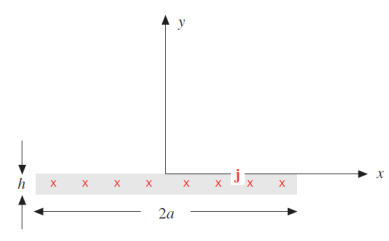
\includegraphics[scale=0.3]{e_8_7_0.png}
\\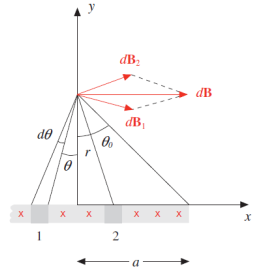
\includegraphics[scale=0.3]{e_8_7_1.png}
\subsubsection*{Formule utilizzate}
\subsubsection*{Soluzione punto a}
La corrente che scorre in un elemento infinitesimo di lamina di larghezza dx è :\\
$di = jhdx$\\
Ogni coppia di elementi infinitesimi, simmetrica rispetto all'asse, contribuirà al campo magnetico con:\\
$d\vec{B} = d\vec{B_1}$$+d\vec{B_2} = 2\frac{\mu_0di}{2\pi r}\cos\theta\vec{u_x}$\\
$y\tan\theta = x\ \rightarrow\ \frac{y}{\cos^2\theta}d\theta = dx\ \rightarrow\ \frac{y}{\cos\theta}d\theta = \cos\theta dx\ \rightarrow\ rd\theta = \cos\theta dx$\\
$d\vec{B} = \frac{\mu_0jh}{\pi}d\theta\vec{u_x}$\\
Integrando su tutta la lampadina si ottiene il campo totale lungo l'asse:\\
$\vec{B} = \int_0^{\theta_M}d\vec{B} = \int_0^{\theta_0}\frac{\mu_0jh}{\pi}d\theta\vec{u_x}=\frac{\mu_0jh}{\pi}\theta_0\vec{u_x}$\\
L'angolo massimo $\theta_0$, corrisponde alla coppia di elementi infinitesimi più lontani dall'asse è:\\
$\theta_0 = arctan\frac{a}{y}$\\
Quindi:\\
$\vec{B} = \frac{\mu_0jh}{\pi}arctan\frac{a}{y}\vec{u_x}$\\
Il momento meccanico che agisce sull'ago magnetico è:\\
$\vec{M} = \vec{m}\wedge\vec{B} = -m\frac{\mu_0jh}{\pi}arctan\frac{a}{y}\vec{u_z}=2.87*10^{-4}\vec{u_z}$[Nm]\\
\subsubsection*{Soluzione punto b}
Vediamo adesso il comportamento di $\vec{B}$ nei limiti per a tendente all'infinito e $2a\ll y$\\
$\lim_{a \to \infty} \vec{B} \tilde{} \lim_{\theta_0\to\frac{\pi}{2}}\vec{B} \tilde{} \frac{\mu_0jh}{2}\vec{u_x}$
\newpage
\end{document}